\documentclass[12pt]{article}
\usepackage[top=1in, bottom=1in, left=1in, right=1in]{geometry}

\usepackage{setspace}
\onehalfspacing

\usepackage[hang,flushmargin]{footmisc} 
% 'hang' flushes the footnote marker to the left,  'flushmargin'  flushes the text as well.

\def\baselinestretch{1}
\setlength{\parindent}{0mm} \setlength{\parskip}{0.8em}

\newlength{\up}
\setlength{\up}{-4mm}

\newlength{\hup}
\setlength{\hup}{-2mm}

\usepackage{amssymb}
%% The amsthm package provides extended theorem environments
\usepackage{amsthm}
\usepackage{epsfig}
\usepackage{times}
\renewcommand{\ttdefault}{cmtt}
\usepackage{amsmath}
\usepackage{graphicx} % for graphics files

% Draw figures yourself
\usepackage{tikz} 

% The float package HAS to load before hyperref
\usepackage{float} % for psuedocode formatting
\usepackage{xspace}

% from Denovo Methods Manual
\usepackage{mathrsfs}
\usepackage[mathcal]{euscript}
\usepackage{color}
\usepackage{array}

\usepackage[pdftex]{hyperref}

\newcommand{\nth}{n\ensuremath{^{\text{th}}} }
\newcommand{\ve}[1]{\ensuremath{\mathbf{#1}}}
\newcommand{\Macro}{\ensuremath{\Sigma}}
\newcommand{\vOmega}{\ensuremath{\hat{\Omega}}}

\begin{document}
\begin{center}
{\bf NE 155, Class 16-18, S14 \\
DE \\ February 28, March 3 and 5 2014}
\end{center}

\setlength{\unitlength}{1in}
\begin{picture}(6,.1) 
\put(0,0) {\line(1,0){6.25}}         
\end{picture}

%-------------------------------------------------------------
I'm going to change the ordering of the syllabus a little bit a drop  a topic. After thinking about it, I think this is overall the best way to go. At the end we'll see if you agree. 

I'm going to skip item \# 3: Point Kinetics and numerical solution of the initial value problem. Instead I'm going to go through a derivation of the transport and diffusion equations more deeply. While this isn't entirely needed, I just feel like it's more satisfying. 

We will then spend a bit more time on the diffusion equation and solution methods (\#4). For the purpose of projects I'm going to switch the ordering of Monte Carlo and Transport Solution methods (\#s 5 and 6). This way you can either do a diffusion solver project or a Monte Carlo project with some information about either method with enough time to do the project. 

Cool?

\section{Transport Equation Redux}

Largely from Lewis and Miller Chp.\ 1 and Duderstadt and Hamilton Chp.\ 4. 

\subsection{Definitions}

Spatial logistics
\begin{itemize}
\item $d\vec{r} = d^3r$ = ordinary volume = $r^2 sin(\theta) d\theta d\phi dr$
%
\item $v$ = speed (scaler)
\item $\vec{v}$ = velocity (vector)
\item $d\vec{v} = d^3v$ = velocity volume = $v^2 sin(\theta')d\theta' d\phi' dr$
\item $v = \sqrt{(2E)/m}$ where $m$ is the rest mass of the particle. Thus, we can relate energy and speed.

\item $\Omega$: unit directional vector in velocity space, $\vec{v} = v\vOmega$
\item $d\vOmega = sin(\theta')d\theta' d\phi' =  d^2\Omega$
%\item thus $d\vec{v} = v^2 dv d\vOmega$
\end{itemize}

\begin{figure}[h!]
\begin{center}
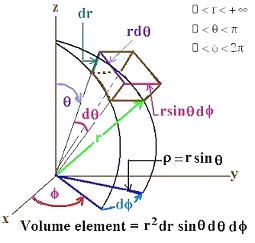
\includegraphics[height=2 in]{VolumeElement}
\end{center}
\end{figure}

Physics terms given possible reactions we're generally going to worry about:
\begin{itemize}
\item total (t): all interactions. Under there there is 
\item scattering (s): a neutron interacts with an atom and bounces off either elastically or inelastically.
\item absorption (a): a neutron is absorbed by a nucleus. If this happens it might
\item fission (f): cause the nucleus to split into 2 pieces, releasing more neutrons
\end{itemize}

\begin{enumerate}
\item \textbf{microscopic x-sec} ($\sigma$, [$cm^2$]): measure of the probability that an incident neutron will collide with a specific nucleus. $\sigma_j$ indicates a specific reaction, e.g.\ $j=f$ is fission.

\item \textbf{macroscopic x-sec} ($\Sigma$ [$cm^{-1}$]): measure of the probability per unit path length that an incident neutron will collide with a target
\[\Sigma_j = \sigma_j N\]
where N is the atomic densigy of the target.

\item \textbf{double-differential scattering x-sec} ($\sigma(E, \vOmega \rightarrow E', \vOmega')dE' d\vOmega'$): measure of the probability that a neutron of energy $E$ and moving in direction $\vOmega$ scatters off of a specific nucleus into energy range $[E', E' + dE']$ and direction range $[\vOmega', \vOmega' + d\vOmega']$.

\item \textbf{fission yield} ($\nu(E)$): is the average number of neutrons released by a fission induced by a neutron of energy E.

\item \textbf{fission spectrum} ($\chi(E)dE$): average \# of fission neutrons produced with energy in $[E, E + dE]$

\item \textbf{particle angular density} ($n(\vec{r}, \vOmega, E, t)d\vec{r} d\vOmega dE dt$): expected number of particles in volume element $d^3r$ at $\vec{r}$ whose energies are in $[E, E + dE]$ and direction of motion is in $[\vOmega, \vOmega + d\vOmega]$ at time $t$

\item \textbf{particle density}: ($N(\vec{r},E,t)d^3r dE$): expected number of particles in $d^3r$ at $\vec{r}$ whose energies are in $[E, E + dE]$ at time $t$.
\[N(\vec{r},E,t)d^3r dE = \int_{4\pi} d\vOmega n(\vec{r}, \vOmega, E, t) \]

\item \textbf{angular flux}: $\psi(\vec{r}, \vOmega, E, t) \equiv v n(\vec{r}, \vOmega, E, t)$ [not a vector]

\item \textbf{scalar flux}: $\phi(\vec{r},E,t) \equiv v N(\vec{r},E,t)$ [not a vector]
\[= \int_{4\pi} d\vOmega \psi(\vec{r}, \vOmega, E, t) \]

\item \textbf{interaction rate density}:
\[\int_{4\pi} d\vOmega \Sigma_j v n(\vec{r}, \vOmega, E, t) = \Sigma_j \phi(\vec{r},E,t)\]
expected number of $j$ reactions per volume per energy at time $t$.

\item \textbf{angular current density}: $\vec{j}(\vec{r}, \vOmega, E, t) = \vec{v} n(\vec{r}, \vOmega, E, t)$ 

Note $\vec{j}(\vec{r}, \vOmega, E, t) \cdot \hat{n} dA dE d\vOmega$ is the expected number of particles crossing $dA$ along $\hat{n}$ with energy in $[E, E + dE]$ and direction in $[\vOmega, \vOmega + d\vOmega]$ at time $t$
\end{enumerate}

%-----------------------------------------
\subsection{Assumptions}
\begin{enumerate}
\item Particles are point objects ($\lambda = h/(mv)$ is small compared to the atomic diameter): its state is fully described by its location, velocity vector, and a given time. This ignores rotation and quantum effects.

\item neutral particles travel in straight lines between collisions.

\item particle-particle collisions are negligible (makes TE linear).

\item material properties are isotropic (generally valid unless velocities are very low).

\item material composition is time-independent.

\item quantities are expected values: fluctuations bout the mean for very low densities are not accounted for.
\end{enumerate}


%-----------------------------------------
\subsection{Derivation}
The TE is a \underline{detailed} balance of the particle population over phase space that is as close to exact as possible. 

DRAW PICTURE

Consider a volume $V$ with surface $S$. For each point $\vec{r} \in S$, let $\hat{n}_S$ be the outward normal vector.

For a given $\vOmega$, define $S^+$ as that part of $S$ for which $\hat{n}_S \cdot \vOmega > 0$ (outgoing particles) and $S^-$ as that part of $S$ for which $\hat{n}_S \cdot \vOmega < 0$ (incoming particles).

Then, for a this volume $V$ for a fixed $E$ and $\vOmega$, the general rate equation can be written for particles satisfying $\vec{r} \in V$, energies in $[E, E+dE]$ and direction $[\vOmega, \vOmega + d\vOmega]$ as:

\hspace*{3 em} \boxed{\text{Rate of change of the particle (neutron) population 
 = rate of production - rate of loss}}

\subsubsection{Rate of Change}
Recall the definition of $n$: expected number of particles in volume element $d^3r$ at $\vec{r}$ whose energies are in $[E, E + dE]$ and direction of motion is in $[\vOmega, \vOmega + d\vOmega]$ at time $t$

To get the rate of change of particles within the volume, we need to integrate over volume and take the derivative with respect to time:

\[\Biggl[ \int_V \frac{\partial}{\partial t} n(\vec{r}, E, \vOmega, t) d\vec{r} \Biggr] dE d\vOmega \]


\subsubsection{Production Mechanisms}

\subsubsection{Loss Mechanisms}




\end{document}